\section{Text Mining Pipeline}
\label{sec:pipeline}
This section describes how the raw data is preprocessed in order to train a classifier that performs NER and NEL on German newspaper articles.
~\\
Preprocesing on Wikipedia dump\\
Explanation of jobs and their runtimes\\
Tools: Stanford CoreNLP (Tokenizer), Apache Lucene (Stemmer)\\
Data structures: Trie (for alias recognition)\\

\subsection{Raw data}
The system uses Wikipedia and Wikidata as data sources to train the classifier that performs NEL. The following will describe both of them.

\subsubsection{Wikipedia}
As project aims on analyzing German newspaper articles, the German Wikipedia provides appropriate training data. It currently consists of more than 3.6 million articles [source]. The articles have 3 main components:
\begin{itemize}
\item Natural language text makes up most of the data.
\item Links to other Wikipedia pages.
\item Structured content, such as infoboxes.
\end{itemize}
The system will train the classifier based on the text and the links. It discards the structured content, as most of it is part of DBpedia [source], which is already included in the company graph [source reference to other BA].\\
For faster processing, the system accesses this data via a dump of the Wikipedia [source link] that consists of XML and Wikimarkup. The whole dump has a size of 15.9 GiB.

\subsubsection{Wikidata}
The German Wikidata [source link] describes the same entities as the German Wikipedia. But in contrast to Wikipedia, it does not provide a textual description but an ontology for them. This includes the class of an entity, which can be a business or an organization [todo concrete identifier]. This information is used to train the classifier only with relevant data.\\
As Wikipedia, the system also accesses the German Wikidata via a dump that is stored as JSON. It has a size of 90.2 GiB.

\subsection{Overview}
The preprocessing of the raw data consists of multiple steps as depicted in Fig.~\ref{fig:job_dependencies}. The system
\begin{itemize}
\item filters the data sources for their relevant content and stores this into tables of an Apache Cassandra database. (Parsing)
\item refines the links within the Wikipedia and counts the references between each alias and entity. (Link analysis)
\item searches for aliases of organizations in the Wikipedia text. (Alias analysis) 
\item analyzes the frequencies of words in the Wikipedia text. (Word analysis)
%- generates features to train the classifier. (Feature generation)
%- trains the classifier. (Classifier training)
%- performs NEL on newspaper articles. (NEL)
\end{itemize}

\begin{figure}[ht]
	\centering
  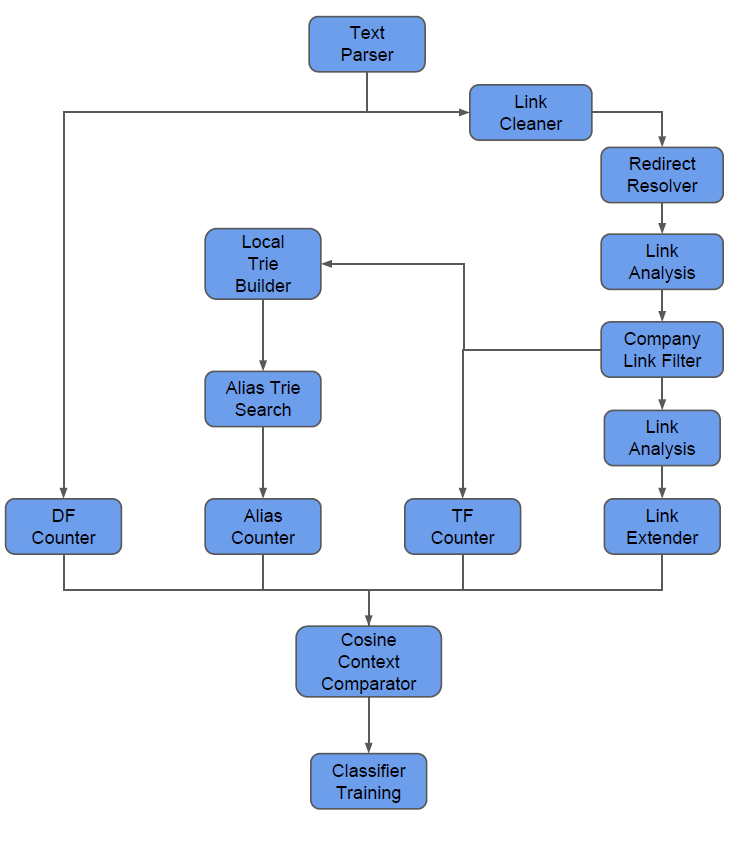
\includegraphics[width=0.7\textwidth]{Graphics/job_dependencies.png}
	\caption{Dependencies between the jobs of the text mining pipeline}
	\label{fig:job_dependencies}
\end{figure}


\subsection{Data preprocessing}
This subsection describes how the presented steps work in detail.

\subsubsection{Parsing}
For each article in Wikipedia, the parsing step converts the Wikimarkup to HTML by means of [source tool]. It then extracts the raw text and saves it into a Cassandra table along with the contained links to other Wikipedia entities.

\subsubsection{Link analysis}
At first, the link analysis step refines the extracted Wikipedia links. This means that it removes links to nonexistent pages and resolves links to redirect pages to their final target pages.\\
Secondly, the link analysis generates statistics about how often a specific alias occurs as a link and which target pages it has how often. For example, the alias "BMW" occurs 5700 times as a link, and directs in 4264 cases to the page "BMW". In only 6 cases, it directs to the page "Berlins Most Wanted". The link analysis also generates these statistics vice versa by counting how often a specific page is linked by which aliases. This means, for example, that the page "BMW" is linked by the alias "BMW" in 4264 cases but only 155 times by "BMW AG". [graphic for this example] These statistics are helpful to identify aliases of organizations, estimate the probability that an alias means an organization (see Sec.~\ref{sec:link_score}) and that it means a specific organization (see Sec.~\ref{sec:page_score}).\\

\subsubsection{Alias analysis}
Most of the links [concrete number] that are contained in Wikipedia are not relevant for the desired company graph, as they do not link to an organization. Wikidata provides an ontology that allows to identify which of Wikipedia's entities is an organization. This could be used to discard all links that do not link to an organization. But instead, the alias analysis uses the statistic from the previous step that lists all occurring aliases for a specific page to find all aliases that link to an organization. Only after it has determined these aliases, the alias analysis removes all those links that have an alias that directs to an organization in no case. In this way, the system retains links that do not link to an organization but have an alias of an organization. Those links are a valuable true negatives that are used to train the classifier that identifies mentions of organizations in raw text later on [reference to classifier training].\\
To gain even more training data for the classifier, the alias analysis builds a trie (a character based prefix tree) that contains all known aliases. It then uses the trie to identify all occurrences of organization aliases in Wikipedia articles that are no links. The alias analysis assumes aliases that also occur as a link in the same article as meaning the same entity. It saves them as so-called extended links, which serve as true positives. If aliases have no corresponding link in the same article, the alias analysis saves them as a so-called trie hit, which serve as true negatives.\\

\subsubsection{Word analysis}
As an alias may have multiple meanings, the classifier requires additional information to disambiguate its occurrences in newspaper articles. A helpful feature is the context of those occurrences (see Sec.~\ref{sec:context_score}), since it strongly depends on their meaning. The classifier therefore needs a way to describe the content of raw text.\\
In NLP, a common approach to evaluate the content of raw text is the bag-of-words model [link]. This model considers a text as a multiset of its contained words, which means a set that may contain words multiple times. Although the order of the words is lost, the model can be used to determine whether different texts describe similar subjects or not. For example, two newspaper articles that contain the words "Automobil" (automobile) and "Ingolstadt" multiple times are likely to both address the German automobile manufacturer "Audi", as its headquarters are located in Ingolstadt.\\
As the last step of the data preprocessing, the word analysis step extracts those bag of words for each Wikipedia article and each context of a link or extended link. We assume that 20 words before as well as after the link occurrence are representative for the meaning of the alias. This bag of words is called the context of the link.\\

\paragraph{Text parser}
\paragraph{Link cleaner}
\paragraph{Redirect resolver}
\paragraph{Link analysis}
\paragraph{Company link filter}
\paragraph{Link extender}
\paragraph{Trie builder}
\paragraph{Alias trie search}
\paragraph{Alias counter}
\paragraph{Document frequency counter}
\paragraph{Term frequency counter}
\paragraph{Cosine context comparator}

\subsection{Classifier training}
details following in the next section